\section{Analoog}
\subsection{De opdracht}
\begin{minipage}{0.45\textwidth}
	Maak een derde orde 0.5dB ripple chebyshev lowpass filter met een $F_C$ van 70Hz. In de doorlaat band 
	moet er met 10dB worden versterkt. Uit de tabel zijn de volgende gegevens te halen.

	\noindent
	Daarnaast moet het filter met de Sallen-key topologie worden gerealiseerd.
\end{minipage}
\hfill
\begin{minipage}{0.45\textwidth}
	\begin{itemize}
		\item In doorlaat +10dB versterking
		\item $\omega_{0_1}=1.0688$ 
		\item $\omega_{0_2}=0.6265$
		\item $\alpha = 0.5861$
		\item $Q=\frac{1}{\alpha}=1.7061$
	\end{itemize} % Gegevens komen uit tabel 8.30 van het boek linear circuit design
\end{minipage}

\subsection{Overdracht bepalen}
\begin{minipage}{0.40\textwidth}
	Door de waardes uit de tabel in te vullen in de standaard formule (zie formule \ref{eq:hs})
	komt daar formule \ref{eq:hsNum} uit.

	\noindent
	H(s) kan worden opgesplitst in een tweede orde deel en een eerste orde deel zie formule \ref{eq:hsSplit}.
	Het opsplitsen van $H(s)$ in $H(s)_1$ en $H(s)_2$ is noodzakelijk voor het goed ontwerpen van het analoge 
	filter.

	\noindent
	Het tweede orde deel heeft de overdracht die te zien is in formule \ref{eq:hs1} en de overdracht van
	het eerste orde	deel is te zien in formule \ref{eq:hs2}
\end{minipage}
\hfill
\begin{minipage}{0.60\textwidth}
	\begin{align}
		H(s)&=\frac{(\omega_{0_1}\cdot\omega_c)^2\cdot\omega_c\cdot\omega_{0_2}}{(s^2+ \alpha \cdot \omega_{0_1} \cdot \omega_c \cdot s + (\omega_{0_1}\cdot\omega_c)^2)\cdot (s + \omega_c \cdot \omega_{0_2})} \label{eq:hs} \\
		H(s)&=\frac{220\, 156.6429\,\cdot\, 275.0335}{(s^2+274.9999\cdot s+220\, 156.6429)(s+275.0335)} \label{eq:hsNum}\\
		H(s)&= H(s)_1 \cdot H(s)_2 \label{eq:hsSplit} \\ 
		H(s)&_1=\frac{(\omega_{0_1}\cdot\omega_c)^2}{s^2+ \alpha \cdot \omega_{0_1} \cdot \omega_c \cdot s + (\omega_{0_1}\cdot\omega_c)^2} \label{eq:hs1} \\ 
		H(s)&_2=\frac{\omega_c\cdot\omega_{0_2}}{s + \omega_c \cdot \omega_{0_2}} \label{eq:hs2} \\ 
	\end{align}
\end{minipage}
 
%$H(s)_1=\frac{220\, 156.6429}{s^2+274.9999s+220\, 156.6429}$
%$H(s)_2=\frac{275.0335}{s+275.0335}$

\subsection{Tweede orde/Sallen-key}
\begin{wrapfigure}[6]{l}{0.25 \textwidth}
	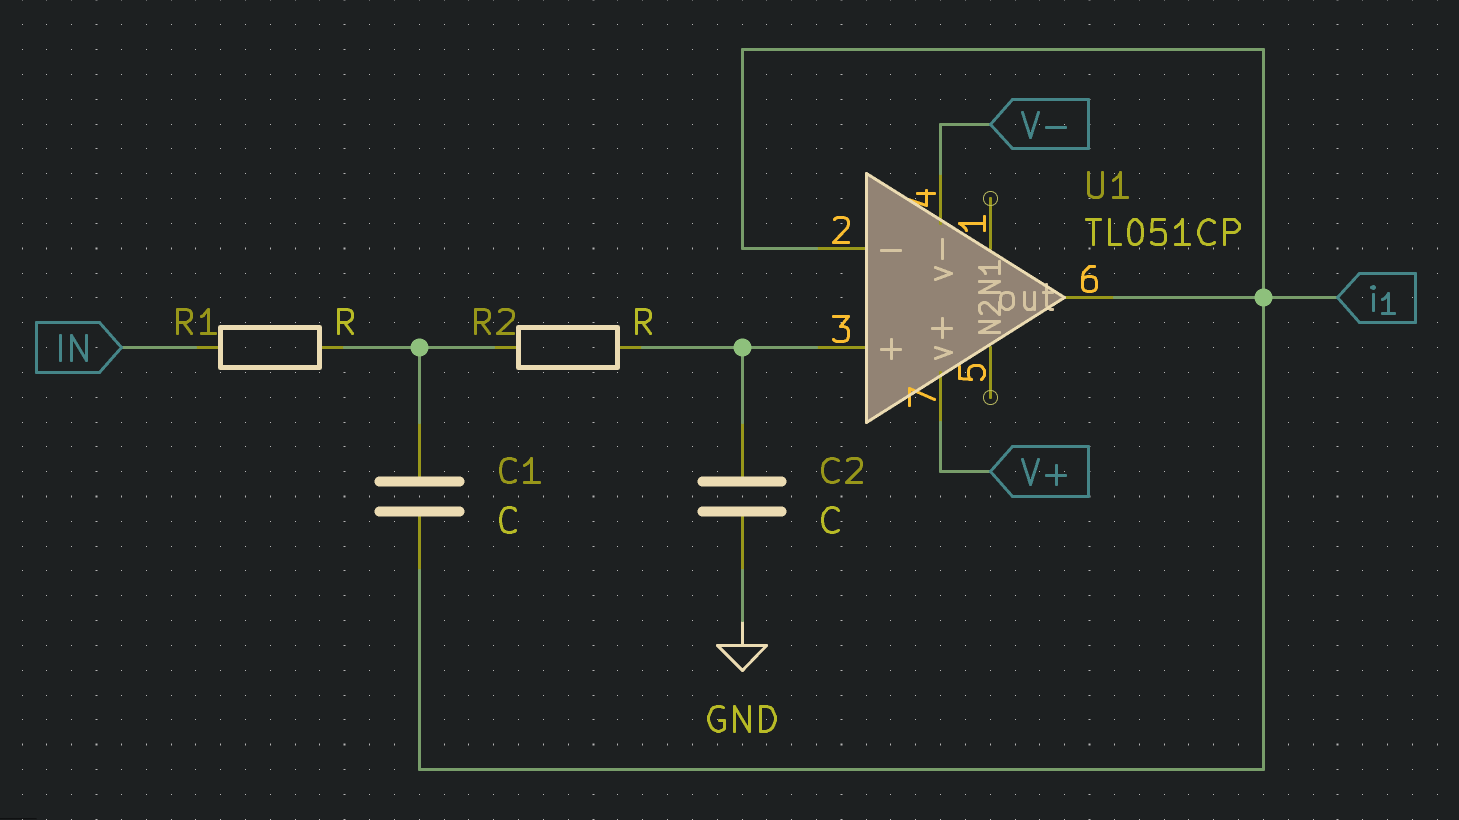
\includegraphics[width=0.9\linewidth]{schematic/sallenkay.png}
	\caption{Sallen-key}
	\label{fig:sallenKey}
\end{wrapfigure}

\vphantom{-}\\
\begin{minipage}{0.37\textwidth}
	Het tweede orde deel van het derde orde filter wordt via de Sallen-key topologie gerealiseerd. In afbeelding \ref{fig:sallenKey} is te zien 
	hoe een laag doorlaat sallen-key filter er uit ziet.
\end{minipage}
\hfill
\begin{minipage}{0.37\textwidth}
	\begin{equation} \label{eq:c1}
		C_1=\frac{2Q}{\omega_c\omega_{0_1}R}
	\end{equation}
	\begin{equation} \label{eq:c2}
		C_2=\frac{1}{2Q\omega_c\omega_{0_1}R}
	\end{equation}
\end{minipage}
\vphantom{-}\\

\noindent
Als $R_1 = R_2$ kan $C_1$ berekend worden met formule \ref{eq:c1} en $C_2$ met formule \ref{eq:c2}.
Voor dit filter is gekozen om voor R $10k\Omega$ te kiezen. Waardoor $C_1=727nF$.

\noindent
727nF is alleen niet een waarde waarin condensatoren worden gemaakt. Door $C_1$ te veranderen naar 750nF 
kan er wel een condensator worden gekocht met de juiste waarde. 

\noindent
Door $C_2$ met formule \ref{eq:c2} uit te rekenen komt $C_2$ uit op een waarde van 62nF, deze waarde is wel direct 
te koop. 

\noindent
Beide waardes zitten alleen niet in de E6/12 reeks en zijn dus aanzienlijk duurder, 
hier gaat een afweging meespelen tussen de prijs van componenten en de kwaliteit van het filter.

\subsection{Eerste orde}
\begin{wrapfigure}[6]{l}{0.25\textwidth}
	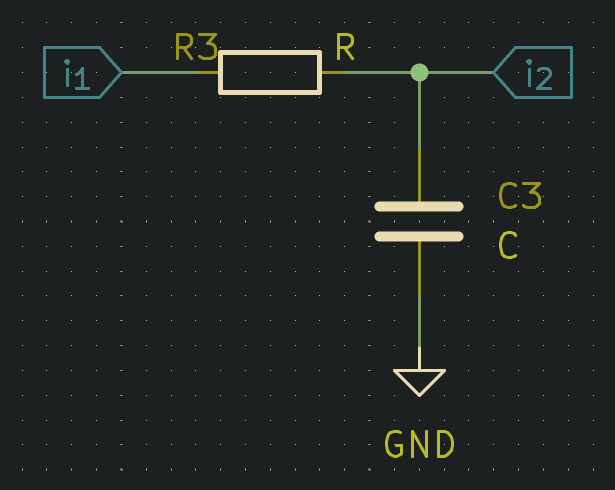
\includegraphics[width=0.9\linewidth]{schematic/rc.png}
	\caption{Eerste orde lp filter}
	\label{fig:lp}
\end{wrapfigure}
\vphantom{-}\\
Een passief eerste orde laag doorlaat filter staat in figuur \ref{fig:lp}. Met formule \ref{eq:rc} is het mogelijk om de verschillende component waardes uit te rekenen 
voor het filter. Wij hebben $C_3=100nF$ gekozen waaruit formule \ref{eq:rcValR} volgt dat 
$R_3=5787\Omega$ dit moet worden afgerond op $5.6k\Omega$ omdat er geen weerstanden beschikbaar zijn met een waarde van $5787\Omega$.

\begin{flushright}
	\begin{minipage}{0.37\textwidth}
		\begin{equation} \label{eq:rc}
			\omega_c*\omega_{0_2}=\frac{1}{R_3C_3}
		\end{equation}
	\end{minipage}
	\begin{minipage}{0.37\textwidth}
		\begin{equation} \label{eq:rcValR}
			R_3=\frac{1}{\omega_c\omega_{0_2}C_3}
		\end{equation}
	\end{minipage}
\end{flushright}
\newpage

\subsection{LTspice}
Het filter dat in afbeelding \ref{fig:filterTotaal} is te zien is gesimuleerd in LTspice. De resultaten van de simulatie zijn te zien
in afbeelding \ref{fig:simRes}.
\begin{figure}[!htb]
	\begin{minipage}{0.45\textwidth}
		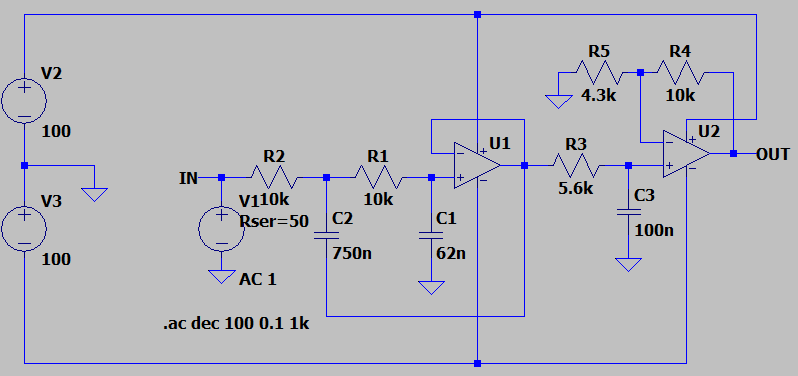
\includegraphics[width=0.9\textwidth]{simulation/schematic.png}
		\caption{Eerste orde lp filter}
		\label{fig:filterTotaal}
	\end{minipage}
	\begin{minipage}{0.45\textwidth}
		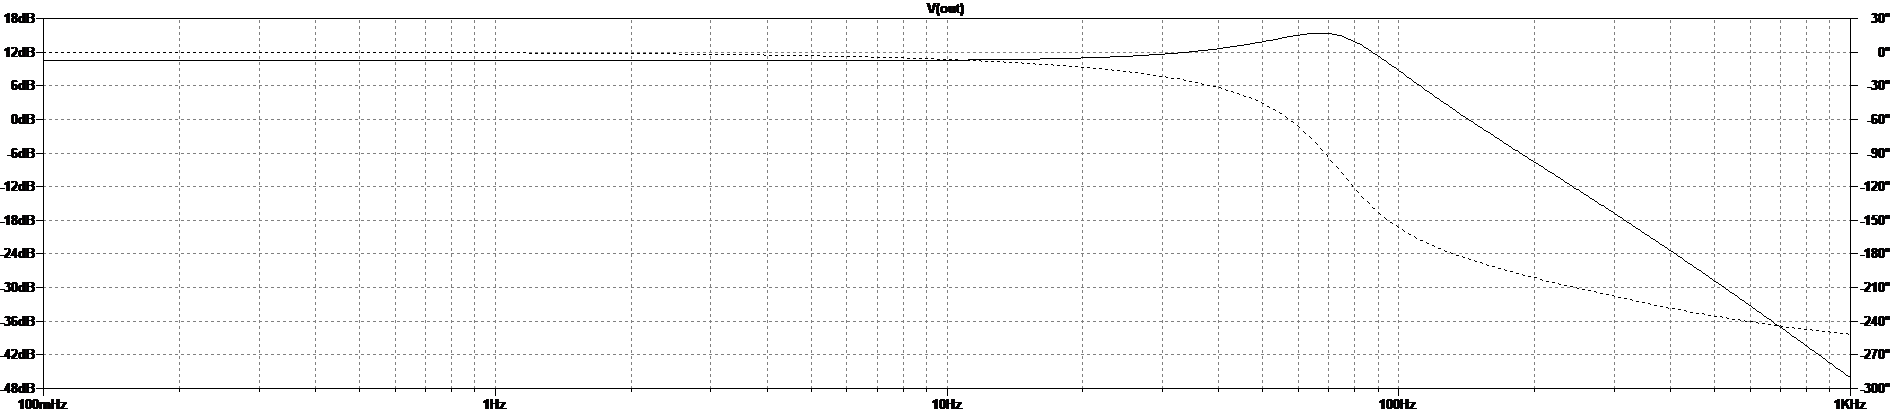
\includegraphics[width=0.9\textwidth, height=100pt]{simulation/Draft2.png}
		\caption{LTspice simulatie}
		\label{fig:simRes}
	\end{minipage}
\end{figure}

\subsection{PCB}
	\begin{wrapfigure}[5]{r}{0.25\textwidth}
		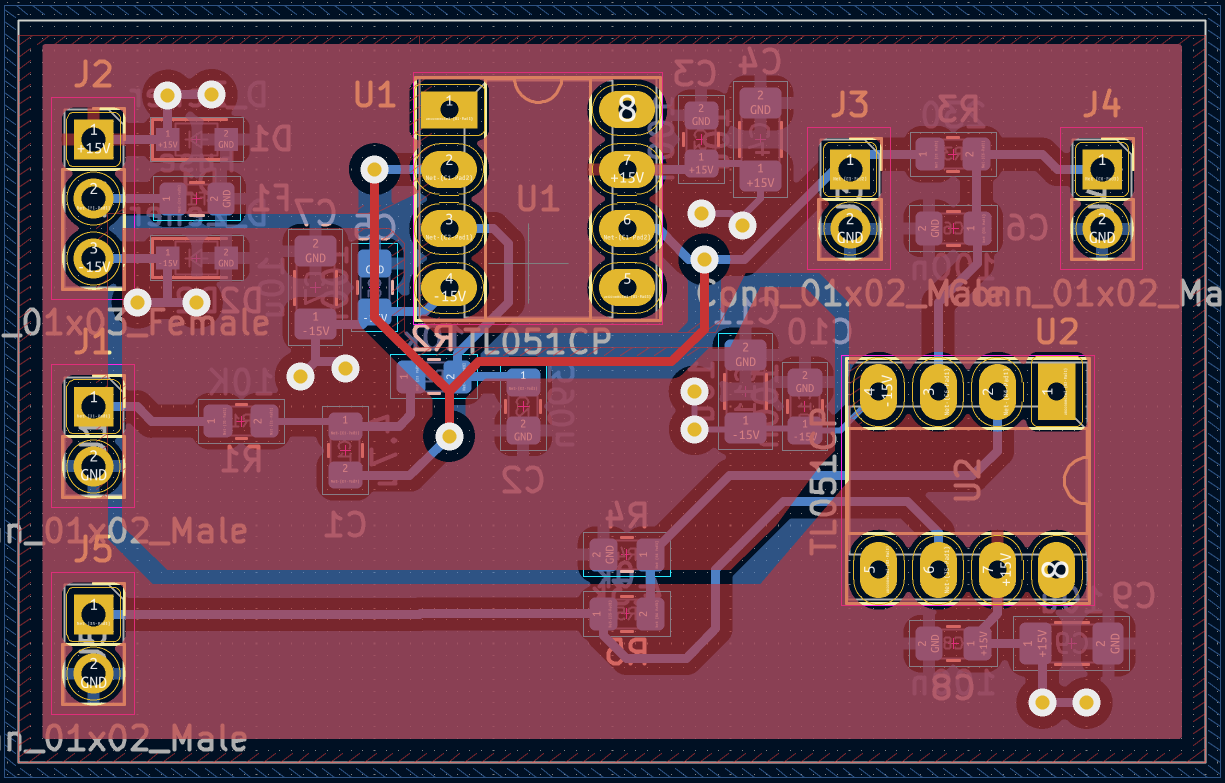
\includegraphics[width=\linewidth, angle=90]{pcb/total.png}
		\caption{Layout}
		\label{fig:pcb:layout}
	\end{wrapfigure}
	Voor deze opdracht hebben wij een pcb ontworpen, op afbeelding \ref{fig:pcb:layout} is de layout te zien. Wij hebben er voor gekozen om een pcb te makenom de 
	parasitaire eigenschappen van onder anderen het breadboard tegen te gaan.

	\noindent
	Bij de layout zijn er nog wel een paar dingen die verbeterd zouden kunnen worden. Een voorbeeld is te zien in afbeelding \ref{fig:pcb:verbeter}
	en in afbeelding \ref{fig:pcb:verbeterde} is te zien hoe dit valt te verbeteren. 
	\begin{figure}[!htb]
		\begin{subfigure}[b]{0.33\textwidth}
			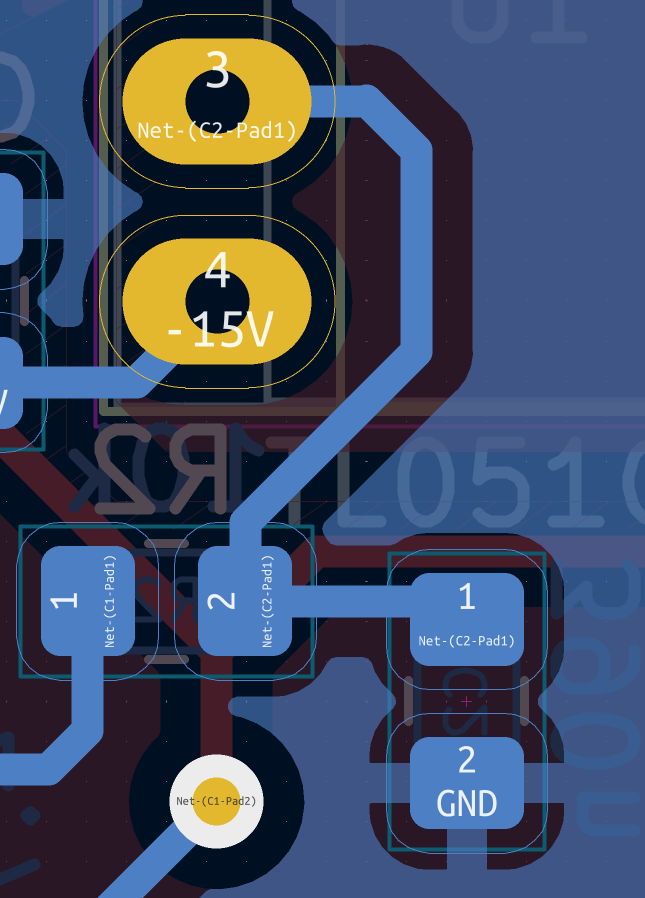
\includegraphics[width=0.5\textwidth, angle=270]{pcb/improvement.png}
			\caption{Dit kan worden verbeterd}
			\label{fig:pcb:verbeter}
		\end{subfigure}
		\begin{subfigure}[b]{0.33\textwidth}
			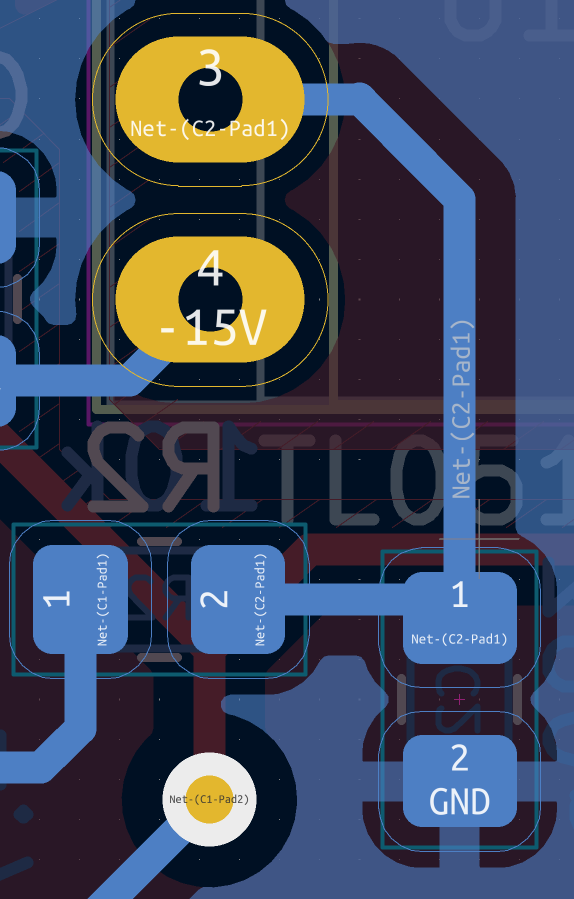
\includegraphics[width=0.5\textwidth, angle=270]{pcb/improved.png}
			\caption{Verbeterd}
			\label{fig:pcb:verbeterde}
		\end{subfigure}
		\caption{verbeter punt}
	\end{figure}

	\noindent
	Op afbeeldingen \ref{fig:pcb:3dBottom} en \ref{fig:pcb:3dTop} is een 3D render te zien van het gemaakte pcb. Bij het ontwerpen van dit pcb is 
	rekening gehouden met alle connectoren aan een kan van de print houden. Daarnaast zijn er nog een paar extra testpoints geplaatst om het debuggen
	van de schakeling makkelijker te maken als deze niet zou werken.
	\begin{figure}[!htb]
		\centering
		\begin{subfigure}[b]{0.45\textwidth}
			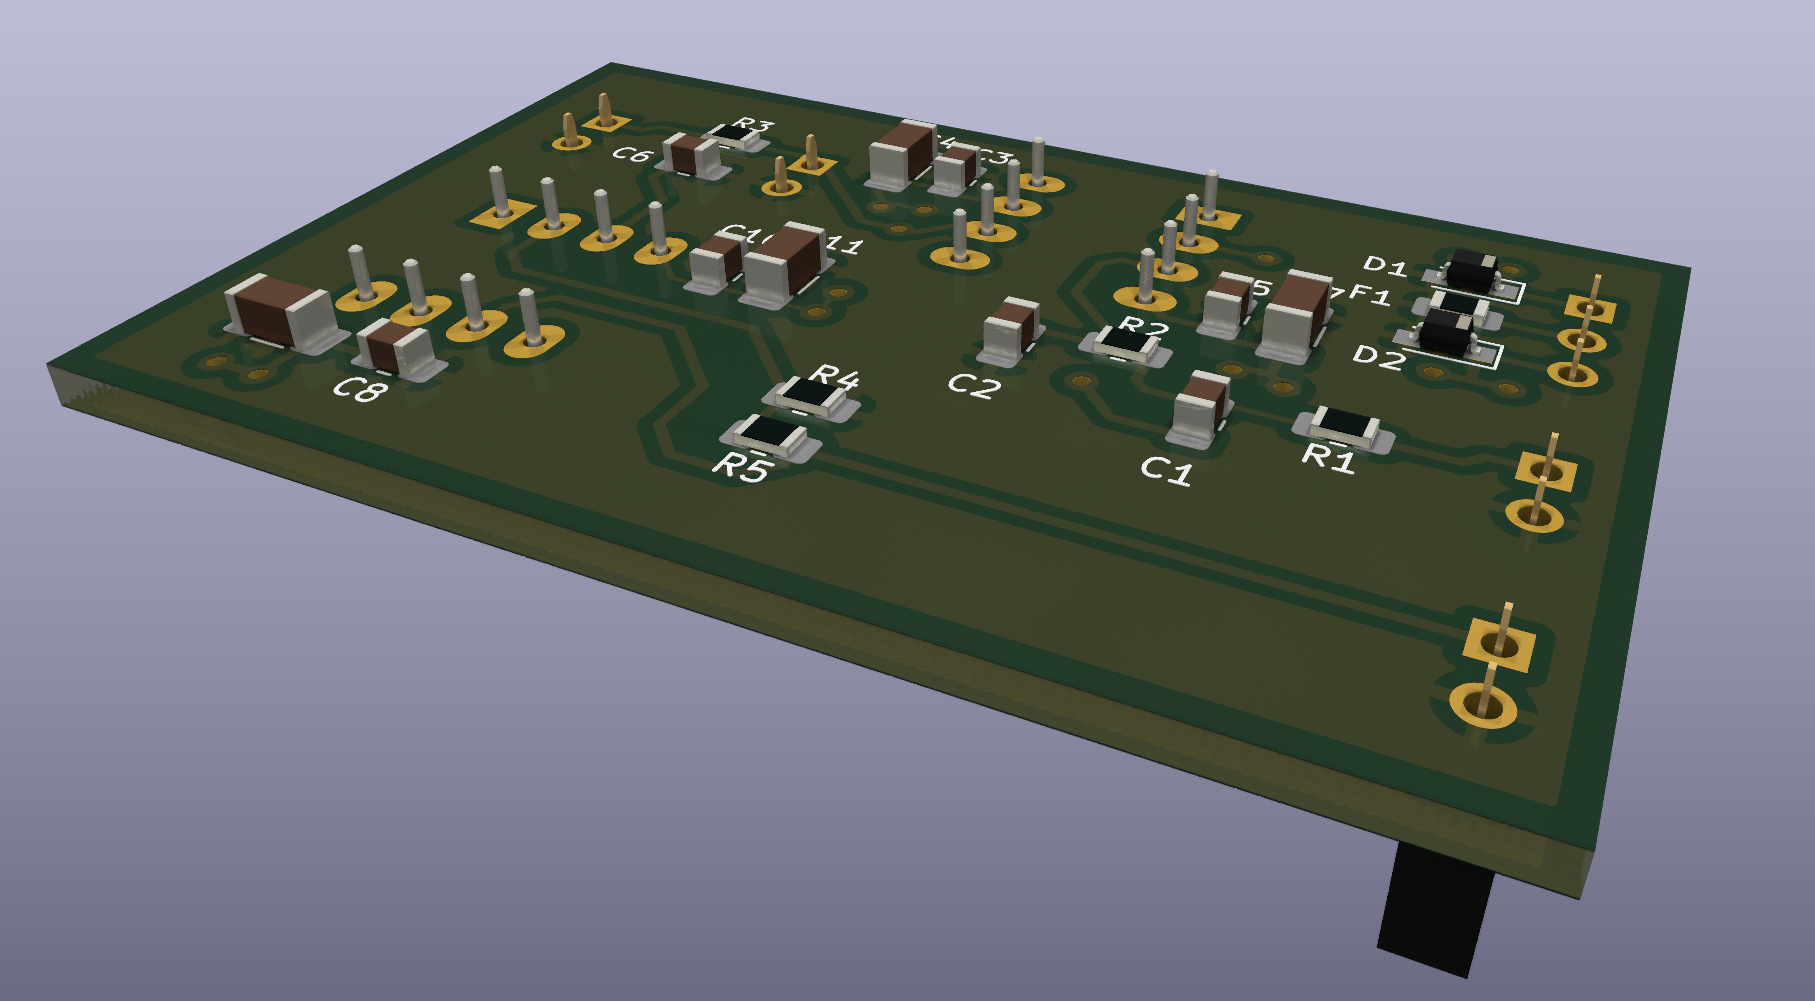
\includegraphics[width=0.7\textwidth]{pcb/bottom.png}
			\caption{onderkant}
			\label{fig:pcb:3dBottom}
		\end{subfigure}
		\begin{subfigure}[b]{0.45\textwidth}
			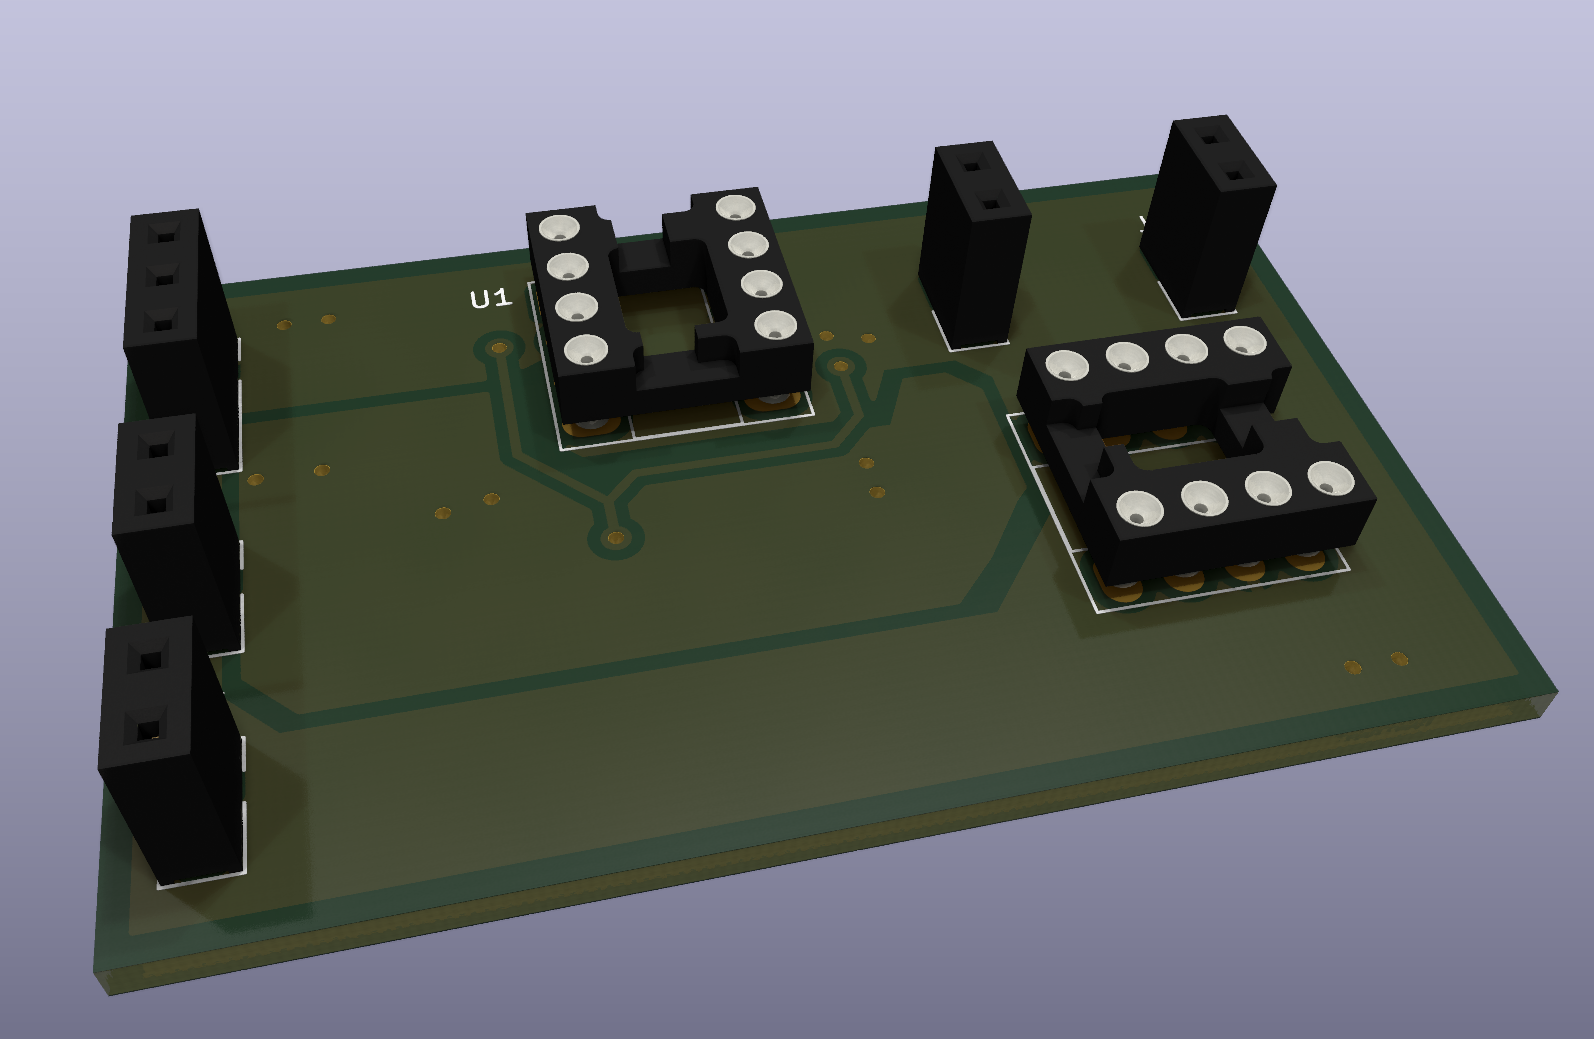
\includegraphics[width=0.7\textwidth]{pcb/top.png}
			\caption{bovenkant}
			\label{fig:pcb:3dTop}
		\end{subfigure}
		\caption{3D renders}
	\end{figure}
	
\newpage


\subsection{Metingen}
\textbf{DISCLAIMER:} Tijdens het berekenen van het filter waren er wat reken fouten gemaakt waardoor het uiteindelijke ontwerp 
niet is opgebouwd met de correcte component waardes zoals ze in dit verslag staan. Het pcb is opgebouwd met de volgende waardes voor de componenten

\noindent
$R_1=R_2=10k\Omega$, $C_1=7.7uF$, $C_2=390nF$, $R_3=230\Omega$, $R_4=4.3k\Omega$ en $R_5=10k\Omega$
\\ 

\noindent
Bij alle metingen is er $\pm 10V$ geleverd ten opzichte van GND. Bij een ingangssignaal van 10Hz $1V_{PP}$ is op afbeelding \ref{fig:amp} te zien wat de output is.
Met een ingangssignaal van 70Hz $1V_{PP}$ is op afbeelding \ref{fig:atten} te zien wat de output is
\begin{figure}[!hbt]
	\begin{subfigure}{0.5\textwidth}
		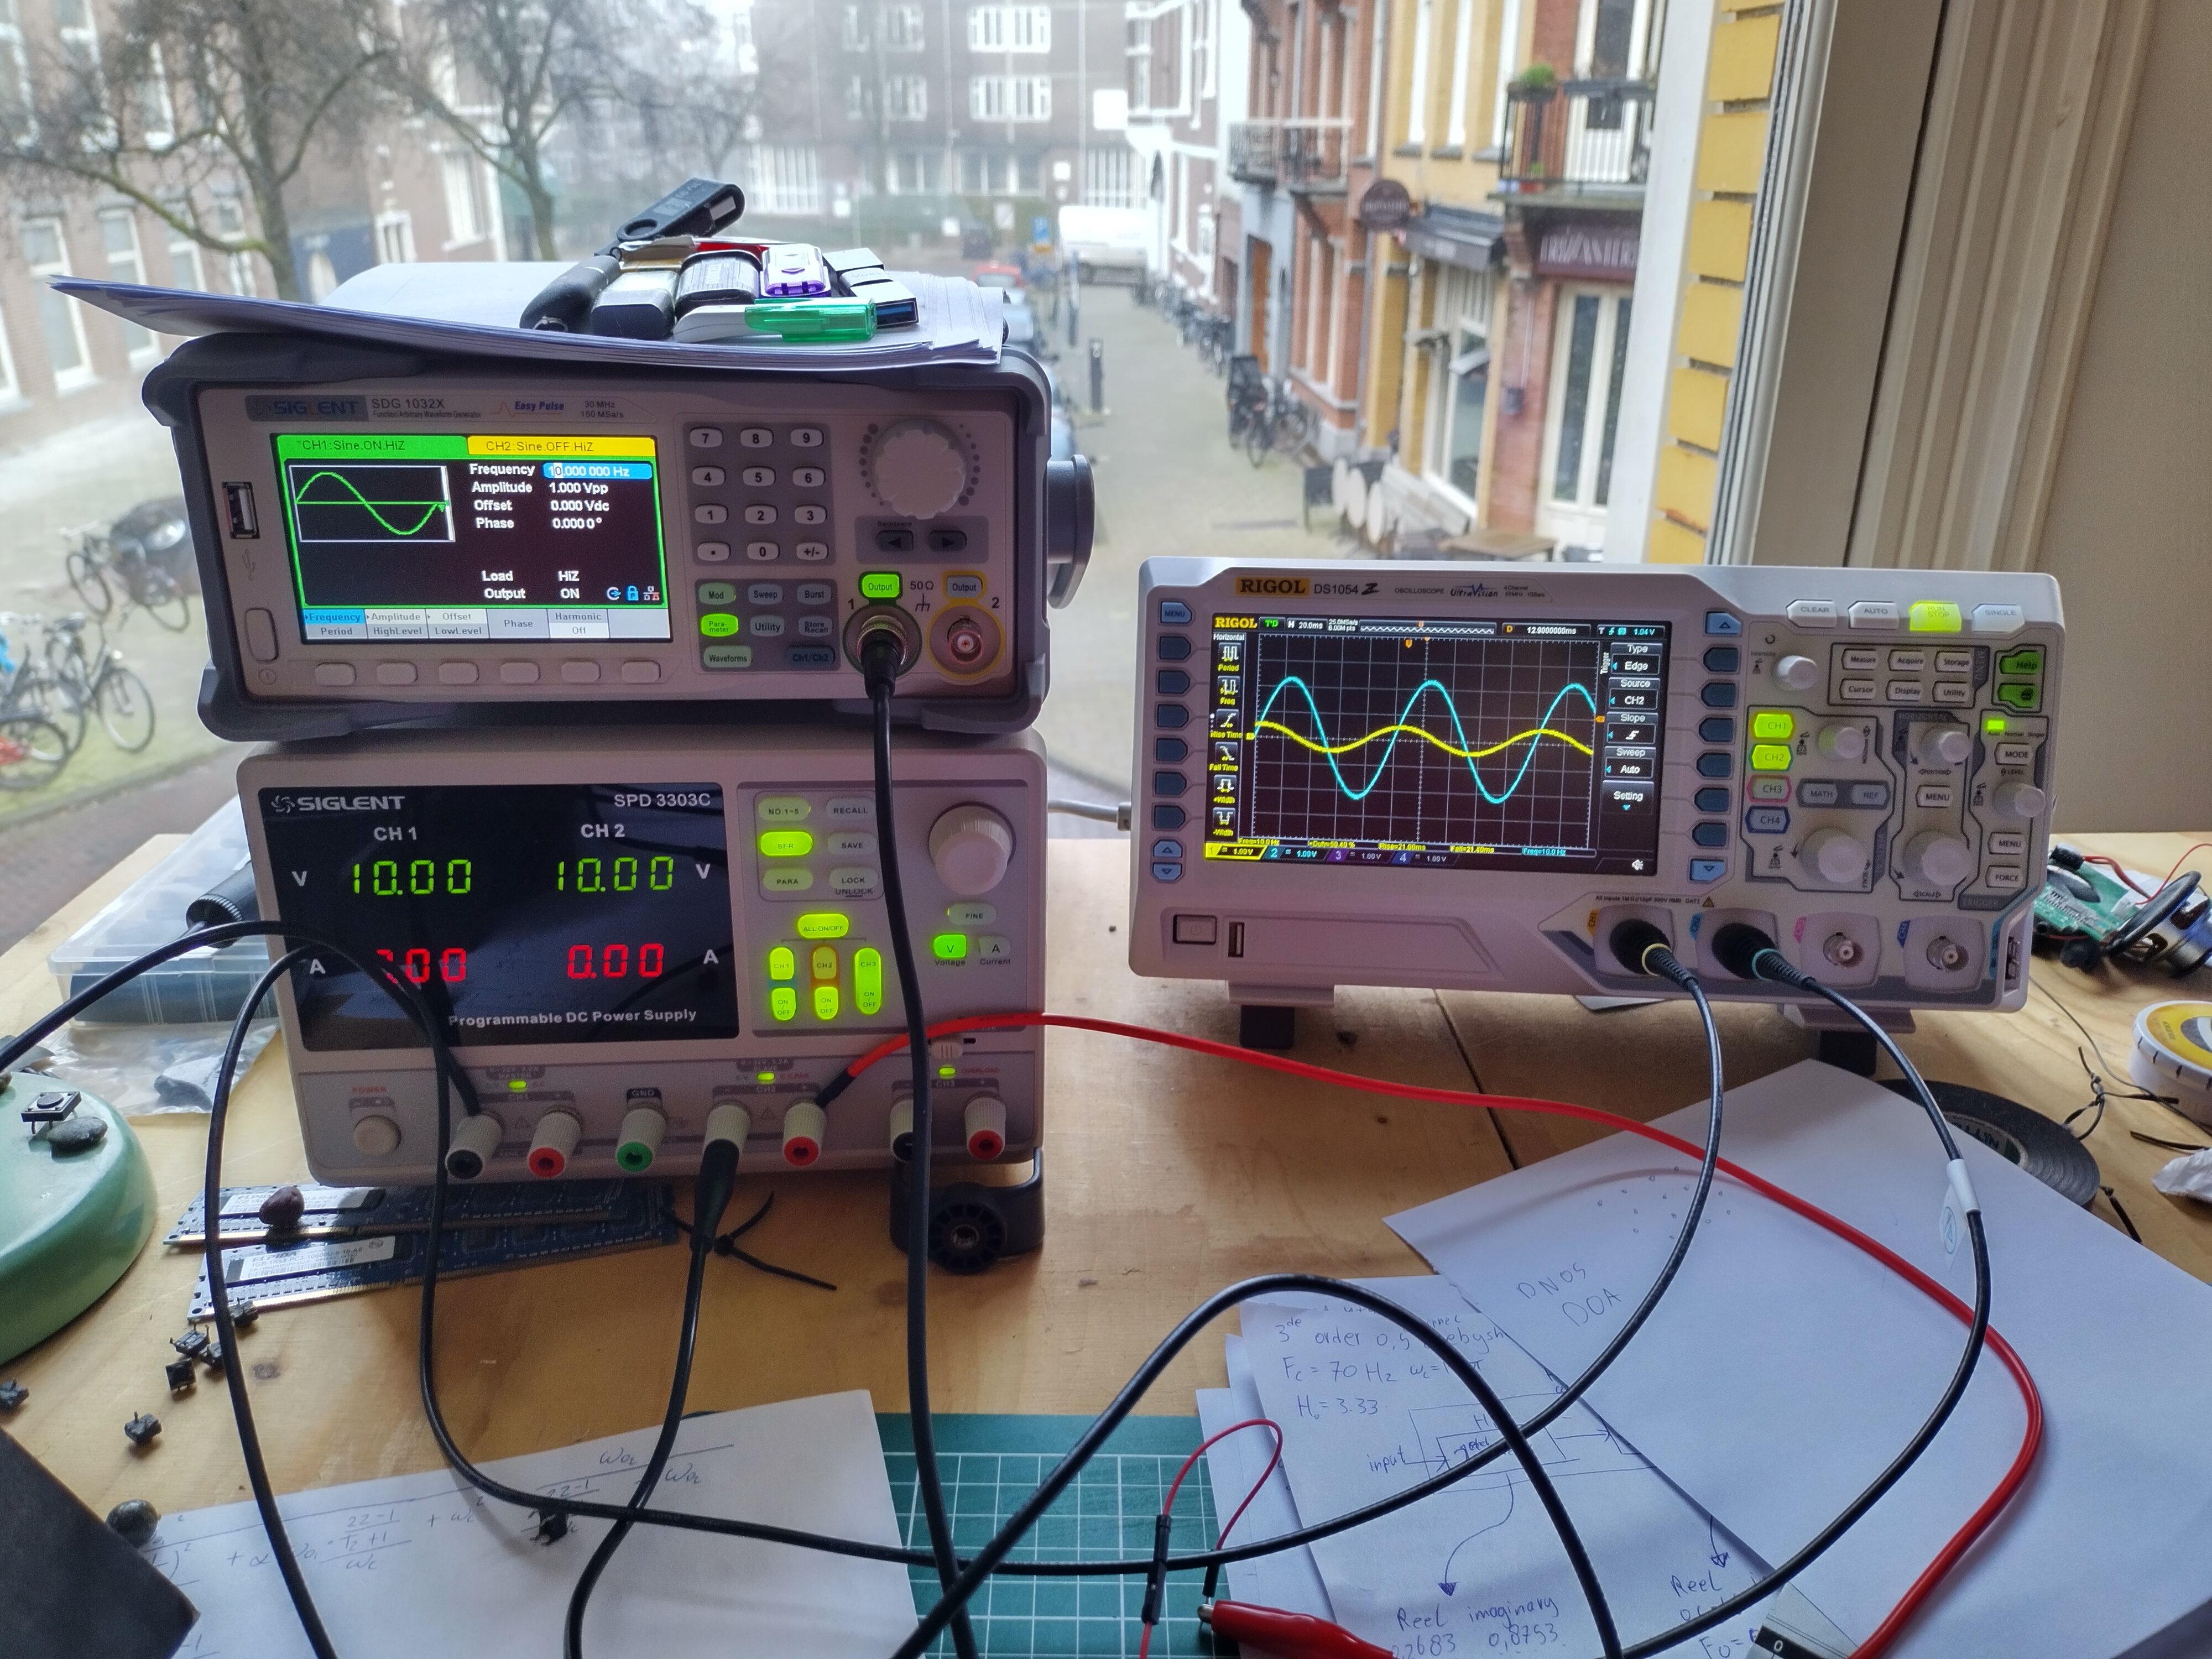
\includegraphics[width=\textwidth]{measurements/versterking.jpg}
		\caption{Versterking}
		\label{fig:amp}
	\end{subfigure}
	\begin{subfigure}{0.5\textwidth}
		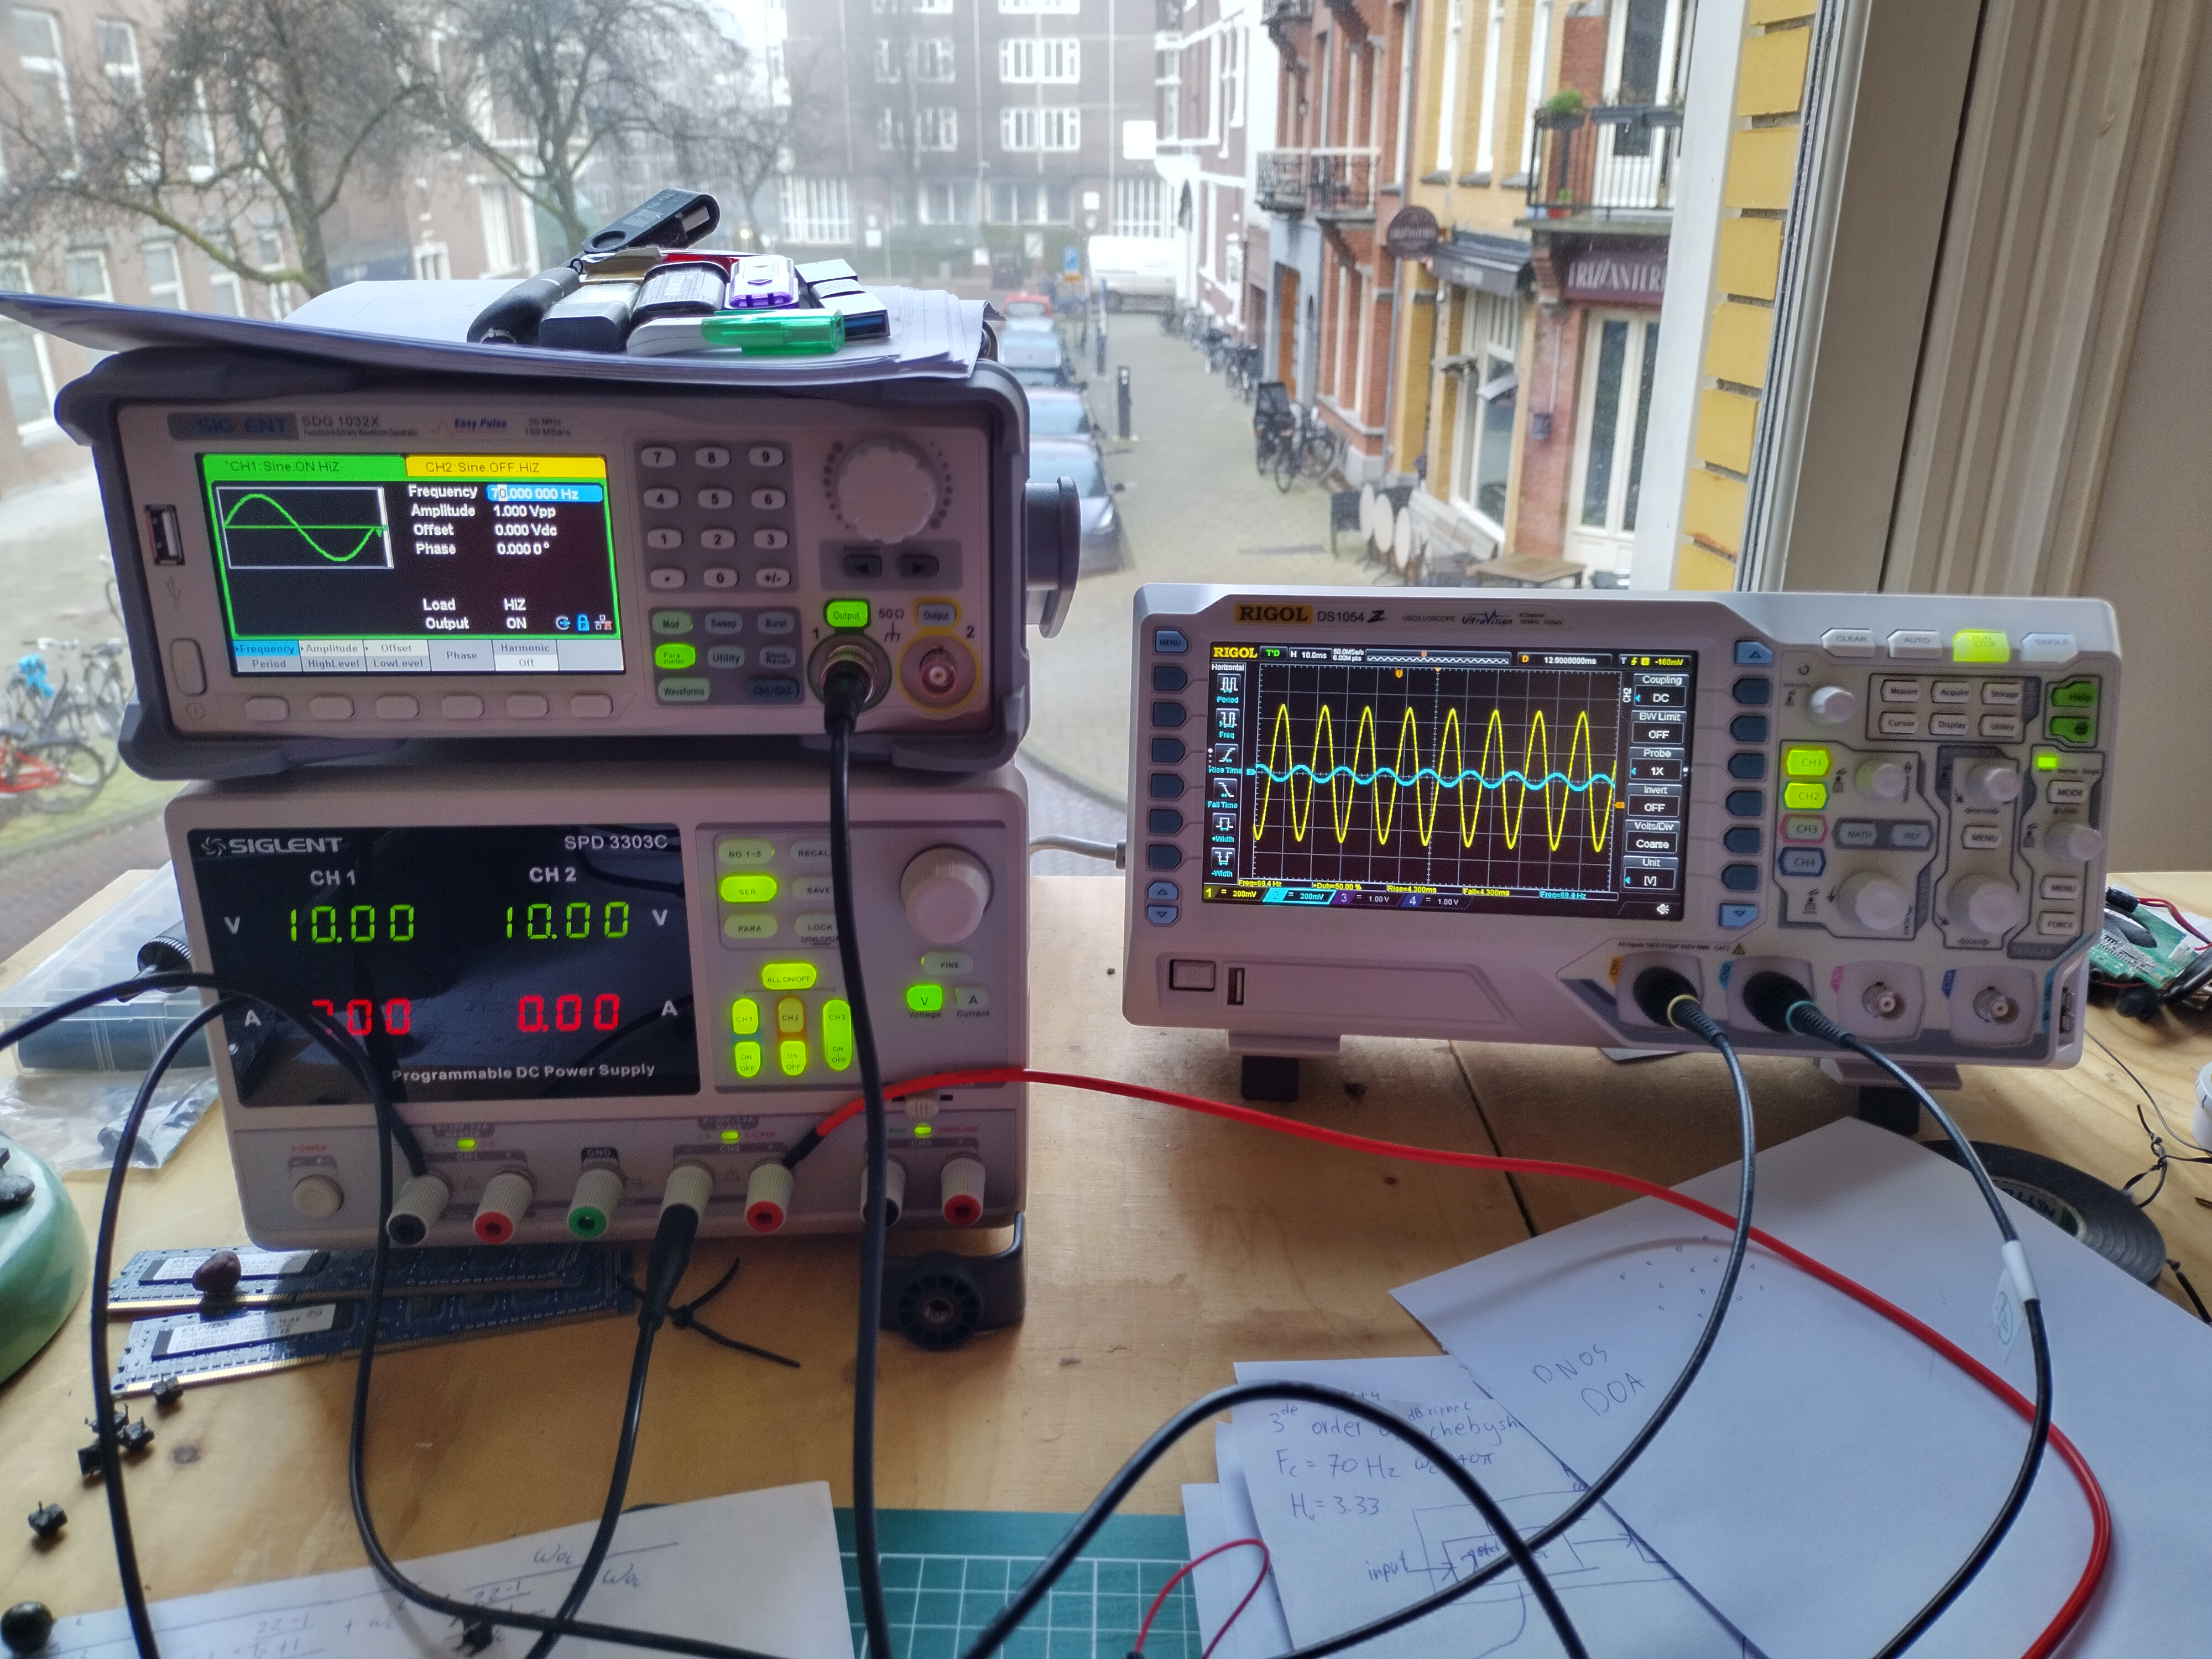
\includegraphics[width=\textwidth]{measurements/demping.jpg}
		\caption{Demping}
		\label{fig:atten}
	\end{subfigure}
	\caption{Meetingen met een oscilloscope}
\end{figure}

\noindent
Het is te zien dat in de doorlaat band het filter met ongeveer 10dB versterkt en in de stopband het signaal dempt. Waar exact het -3dB punt ligt is 
lichtelijk verschoven naar een lagere frequentie. Dit komt zoals in de disclaimer van dit stuk al staat er met verkeerde component waardes is gemeten.